\documentclass[UTF8]{ctexart}

\usepackage{ctex}
\CTEXsetup[format={\Large\bfseries}]{section}
\usepackage[top=28mm,bottom=28mm,left=15mm,right=15mm]{geometry}

\usepackage{fancyhdr}
\fancypagestyle{plain}{\pagestyle{fancy}}
\pagestyle{fancy}
\lhead{\kaishu 清华大学药学院药理毒理实验}
\newcommand{\numOfReport}[1]{\rhead{\kaishu 实验报告#1}}

\usepackage{fontspec}
\usepackage{wasysym}
\setCJKmainfont[AutoFakeBold={2}]{STZhongsong}
\setCJKmonofont{STZhongsong}

\usepackage{float}
\usepackage{booktabs}
\usepackage{tabularx}
\usepackage{array}
\usepackage{amsmath}
\usepackage{amsfonts}
\usepackage{amssymb}
\usepackage[figuresleft]{rotating}
\usepackage[para]{threeparttable}
\newcommand\info[2][40mm]{\underline{\makebox[#1][c]{#2}}}
\newcommand{\infoTable}[7]{
    \renewcommand\arraystretch{1.4}
    \begin{table}
        \begin{tabularx}{\textwidth}{
        >{\hsize=0.6\hsize\linewidth=\hsize}X
        >{\hsize=0.6\hsize\linewidth=\hsize}X
        >{\hsize=2.0\hsize\linewidth=\hsize}X
        >{\hsize=0.8\hsize\linewidth=\hsize}X
        }
            天气:\info[14mm]{#1} & 温度:\info[14mm]{#2 $^{\circ}\text{C}$} & 湿度:\info[14mm]{#3 $\%$} & 日期:#4\\
            姓名:\info[14mm]{#5} & 班级:\info[14mm]{#6} & 同组人:\info[70mm]{#7} & 
        \end{tabularx}
    \end{table}
}
\newcommand\columnC{\centering\arraybackslash}
\newcommand\columnL{\raggedright\arraybackslash}
\newcommand\columnR{\raggedleft\arraybackslash}

\usepackage{svg}
\usepackage{pdfpages}
\title{华法林与肝素抗凝血作用观察}
\author{}
\numOfReport{六}

\begin{document}
\infoTable{晴}{16}{70}{10/30/2024}{何昱晖}{药3}{荣子健、马逸然、赵方一澜}
\date{}
\maketitle

\section{实验目的和原理}

\subsection{实验目的}

\begin{itemize}
    \item [(1)] 学习抗凝血药物的筛选方法;
    \item [(2)] 了解常用抗凝血药物的分类及机制;
    \item [(3)] 观察华法林与肝素的抗凝血作用。
\end{itemize}

\subsection{实验原理}

抗凝血药物(anticoagulant drugs)可用于防止血管内栓塞或血栓形成的疾病,预防中风或其他血栓性疾病。抗凝血药物是通过影响凝血过程中的某些凝血因子阻止凝血过程的药物。正常人由于有完整的血液凝固系统和抗凝及纤溶系统,所以血液在血管内既不凝固也不出血,始终自由流动完成其功能,但当机体处于高凝状态或抗凝状态及纤溶减弱时,则发生血栓栓塞性疾病。临床常用的抗凝血药物包括:非肠道用药抗凝剂(如肝素)、香豆素抗凝血剂类(如华法林)、抗血小板凝集药物(如阿司匹林)、蛇毒溶栓剂(如去纤酶、抗栓酶),以及某些新型口服抗凝药物(如阿哌沙班、达比如群酯)等。

其中华法林(warfarin)是通过抑制维生素 K 参与的凝血因子在肝脏中的合成,从而产生抗凝血作用。凝血因子 \uppercase\expandafter{\romannumeral 2}、\uppercase\expandafter{\romannumeral 7}、\uppercase\expandafter{\romannumeral 9}、\uppercase\expandafter{\romannumeral 10}、蛋白 C 和蛋白 S 在合成后经由维生素 K 依赖的羧化酶将氨基末端谷氨酸羧基化转化为 $\gamma$-羧基谷氨酸,其促凝血活性提高 1000 倍,失活的维生素 K 在环氧化物还原酶的作用下成为还原性维生素 K,参与到凝血因子 \uppercase\expandafter{\romannumeral 2}、\uppercase\expandafter{\romannumeral 6}、\uppercase\expandafter{\romannumeral 9}、\uppercase\expandafter{\romannumeral 10}、蛋白 C 和蛋白 S 的羧化,减少活性凝血因子的产生,达到抗凝血作用。华法林的起效时间与血浆中凝血因子 \uppercase\expandafter{\romannumeral 2}、\uppercase\expandafter{\romannumeral 6}、\uppercase\expandafter{\romannumeral 9}、\uppercase\expandafter{\romannumeral 10} 的半衰期相关,一般为 $18\sim 24\text{h}$。主要用于防治血栓栓塞性疾病。

肝素(Heparin)能干扰血凝过程的许多环节,在体内外都有抗凝血作用。其作用机制比较复杂,主要通过与抗凝血酶 \uppercase\expandafter{\romannumeral 3}(AT-\uppercase\expandafter{\romannumeral 3})结合,而增强后者对活化的 \uppercase\expandafter{\romannumeral 2}、\uppercase\expandafter{\romannumeral 9}、\uppercase\expandafter{\romannumeral 10}、\uppercase\expandafter{\romannumeral 11} 和 \uppercase\expandafter{\romannumeral 12} 凝血因子的抑制作用,其后果涉及组织血小板凝集和破坏、妨碍凝血激活酶的形成、阻止凝血酶原变为凝血酶,抑制凝血酶,从而妨碍纤维蛋白原变成纤维蛋白,从而发挥抗凝作用。

药物的抗凝血作用,教学上通常以毛细玻璃管和载玻片法观察凝血时间长短来衡量,也有采用试管法来测定凝血时间。科研上多采用凝血分析仪测定凝血酶原时间(PT
)、活化部分凝血活酶时间(APTT)、凝血酶时间(TT)、纤维蛋白原(FIB)。以毛细玻璃管和载玻片法测定药物抗凝作用时,凝血时间是指血液流出体外时至凝固时所需的时间。当血液接触毛细玻璃管或载玻片时,外源性凝血系统启动,在一定时间,玻璃管折断处或者载玻片表面出现丝状物。

\section{实验材料}

\begin{itemize}
    \item 实验动物:ICR 小鼠,雄性,$18\sim 22\text{g}$;
    \item 药品和试剂:$0.25\%$ 华法林钠溶液、$0.5\%$ 肝素钠溶液、生理盐水;
    \item 实验器材:注射器(0.1mL)、小鼠灌胃器、毛细玻璃管(内径 1mm、长 10cm)、载玻片、眼科弯镊、大头针、计时器。
\end{itemize}

\section{实验方法}

\subsection{实验内容1:观察华法林的抗凝血作用}

\begin{itemize}
    \item [1] 每组取\textbf{6只}小鼠,称重,标记。实验组3只灌胃给予 $0.25\%$ 华法林钠溶液($0.1\text{mL}/10\text{g}$);对照组3只灌胃给予等体积生理盐水($0.1\text{ml}/10\text{g}$),每天给药一次,连续给药3天;
    \item [2] 第三天,实验组及对照组小鼠分别灌胃 $0.5\sim 1\text{h}$ 后,采用毛细玻璃管和载玻片法测定凝血时间。
\end{itemize}

\subsection{实验内容2:观察肝素的抗凝血作用}

\begin{itemize}
    \item [1] 每组取\textbf{6只}小鼠,称重,标记。实验组3只腹腔注射等体积生理盐水($0.10\text{mL}/10\text{g}$);
    \item [2] 腹腔注射 15min 后,采用毛细玻璃管法和载玻片法测定凝血时间。
\end{itemize}

\subsection{凝血时间测定方法}

\begin{itemize}
    \item [1] 毛细玻璃管:用内径 1mm 毛细玻璃管插入小鼠\textbf{眼内肌球后静脉丛},深约 $3\sim 5\text{mm}$,轻轻转动,待血液充满毛细玻璃管后迅速拔出,并启动秒表开始计时。每隔 30s 折断两端毛细管 $3\sim 5\text{mm}$,并缓慢向左右拉开,观察折断处是否有血凝丝,至血凝丝出现为止,计算从毛细玻璃管采血至出现凝血丝的时间,即为凝血时间,毛细玻璃管两端数据的平均值即为该小鼠的凝血时间。也可以采用割小鼠尾静脉的方法获得血液。
    \item [2] 载玻片法:用眼科弯镊迅速摘去小鼠一侧眼球,即有血液流出,于载玻片两端各第一滴血,两滴血的血滴\textbf{直径应接近},立即用秒表计时,每隔 20s 用清洁大头针\textbf{自血滴边缘向里轻轻挑动一次,并观察有无血丝挑起}。从采血开始至挑起血丝起止,所用时间即为凝血时间,另一端血滴供复验,\textbf{取两个血滴凝固时间的平均值}为该小鼠的凝血时间。
\end{itemize}

注意事项:

\begin{itemize}
    \item [1] 凝血时间可受室温影响,温度过低时凝血时间缩短;
    \item [2] 毛细玻璃管法中所用的玻璃管内径最好为 1mm,并且均匀一致,毛细玻璃管在采血后不宜长时间拿在手中,以免体温影响凝血时间;
    \item [3] 载玻片法中每次挑血滴时,应控制挑动次数,且不应从各个方向多次挑动,以免加快纤维蛋白的形成。
\end{itemize}

\section{实验结果}

\begin{table}[h]
    \centering
    \begin{threeparttable}[b]
        \caption{抗凝血药物对小鼠凝血时间的影响}
        \quad

        \begin{tabularx}{\textwidth}{
            >{\columnC\hsize=1\hsize\linewidth=\hsize}X
            >{\columnC\hsize=1\hsize\linewidth=\hsize}X
            >{\columnC\hsize=1\hsize\linewidth=\hsize}X
            >{\columnC\hsize=1\hsize\linewidth=\hsize}X
            >{\columnC\hsize=1\hsize\linewidth=\hsize}X
        }
            \toprule[1.5pt]
            药物 & 平均毛细玻璃管凝血时间\tnote{1} & 与对照组统计学差异的 $p$ 值 & 平均载玻片法凝血时间\tnote{1} & 与对照组统计学差异的 $p$ 值\\
            \midrule
            华法林钠(实验组) & $457.50\pm 206.46$ & $2.72\times 10^{-5}$ & $586.17\pm 428.00$ & $4.91\times 10^{-4}$\\
            \midrule
            生理盐水(对照组) & $88.44\pm 42.17$ & / & $84.33\pm 36.00$ & /\\
            \midrule[1.2pt]
            肝素钠(实验组) & $186.44\pm 165.56$ & 0.4152 & $186.44\pm 160.41$ & 0.1175\\
            \midrule
            生理盐水(对照组) & $110.80\pm 131.27$ & / & $111.72\pm 129.54$ & /\\
            \bottomrule[1.5pt]
        \end{tabularx}
        \begin{tablenotes}
            \item [1] 单位 s
        \end{tablenotes}
    \end{threeparttable}
\end{table}

\begin{figure}[h]
    \centering
    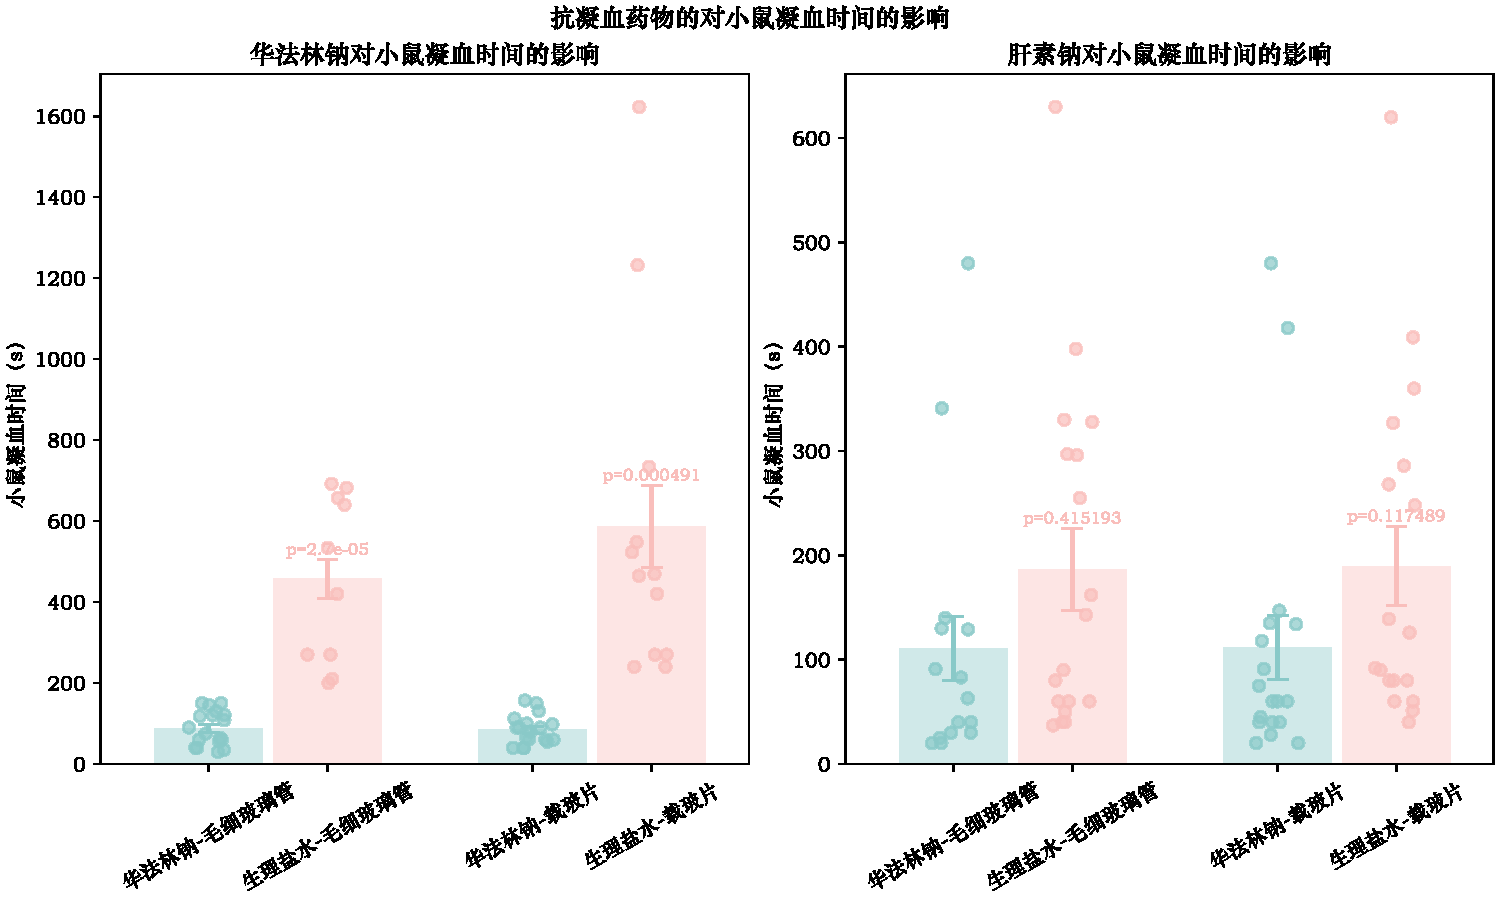
\includegraphics[scale=0.53]{figure-6_svg.pdf}
    \caption{抗凝血药物对小鼠凝血时间影响图}
\end{figure}

\section{课后思考题}

\begin{itemize}
    \item [1] 临床常用的抗凝血药物有哪些?作用机制分别是什么?

    \begin{itemize}
        \item \textbf{凝血酶间接抑制剂}:肝素、低分子肝素(尹诺肝素、那曲肝素、达肝素等)。机理为肝素与抗凝血酶 \uppercase\expandafter{\romannumeral 3}(AT \uppercase\expandafter{\romannumeral 3})结合,形成肝素-AT \uppercase\expandafter{\romannumeral 3} 复合物,增强抗凝血酶 \uppercase\expandafter{\romannumeral 3} 活性数百倍,抗凝血酶 \uppercase\expandafter{\romannumeral 3} 使凝血因子灭活,如凝血酶 \uppercase\expandafter{\romannumeral 2}a、\uppercase\expandafter{\romannumeral 10}a、\uppercase\expandafter{\romannumeral 9}a、\uppercase\expandafter{\romannumeral 12}a、\uppercase\expandafter{\romannumeral 11}a 等;
        \item \textbf{维生素 K 拮抗剂}:香豆素及其衍生物、华法林。机理为使维生素 K 失活,从而干扰维生素 K 依赖的凝血因子包括 \uppercase\expandafter{\romannumeral 2}、\uppercase\expandafter{\romannumeral 12}、\uppercase\expandafter{\romannumeral 9}、\uppercase\expandafter{\romannumeral 10} 的合成;
        \item \textbf{凝血酶直接抑制剂}:水蛭素及其衍生物、比伐卢定、达比加群。机理为直接与凝血酶 \uppercase\expandafter{\romannumeral 2}a 结合形成复合体,使凝血酶灭活;
        \item \textbf{\uppercase\expandafter{\romannumeral 10}a 抑制剂}:利伐沙班、依度沙班、阿哌沙班等。机理为抑制凝血因子 \uppercase\expandafter{\romannumeral 10}a。
    \end{itemize}

    \item [2] 华法林过量服用会导致什么后果?如何进行解救?

    过量服用会导致皮肤粘膜的出血,严重者会造成颅内及内脏出血。可给予维生素 K 对抗华法林进行解救。

    \item [3] 肝素过量服用引起的自发性出血,用什么药物进行解救?

    可应用鱼精蛋白缓慢静脉注射予以中和。
\end{itemize}

\end{document}